\documentclass[a4paper]{article}
\usepackage[francais]{babel} % Le package de Babel pour ecrire en
\usepackage[top=1in, bottom=1.25in, left=1.4in, right=1.4in]{geometry}
%                              % francais;
\usepackage{eurosym}
\usepackage[utf8]{inputenc}%
\usepackage[T1]{fontenc}%
\usepackage[babel=true]{csquotes}
\usepackage{authblk}
\usepackage{url} %
% \usepackage{hyperref} %
% %
% \hypersetup{ %
%   colorlinks=true, %
%   linkcolor=black, %
%   citecolor=black, %
%   urlcolor=black,%
% }%
%

% \usepackage[disable]{todonotes} % notes not showed
\usepackage[draft]{todonotes}   % notes showed

\renewcommand\Authands{, et }

\usepackage{fancyhdr}
\pagestyle{fancy}
\fancyhf{}
\chead{Louis Béziaud, Noé Brucy, Joris Duguépéroux, Antonin Voyez}
\cfoot{\thepage}

\usepackage{pdfpages}

\title{\Huge\textbf{Quoi\(\mid\)ProCo}}

\usepackage[pdftex,
            pdfauthor={Antonin Voyez, Noé Brucy, Louis Béziaud, Joris Duguépéroux},
            pdftitle={Quoi|ProCo},
            pdfsubject={Quoi|ProCo},
            pdfkeywords={},
            pdfproducer={},
            pdfcreator={}]{hyperref}

\author[1,2]{Louis Béziaud}
\author[1,2]{Noé Brucy}
\author[1,2]{Joris Duguépéroux}
\author[1]{Antonin Voyez}

\affil[1]{Université Rennes 1 \protect\\
  \texttt{prénom.nom@etudiant.univ-rennes1.fr}}
\affil[2]{École normale supérieure de Rennes \protect\\
  \texttt{prénom.nom@ens-rennes.fr}}
\affil[ ]{\par\emph{Joris Duguépéroux est porteur du projet}}

\date{}

\begin{document}


\maketitle

\section*{Pitch du projet}

Dans le cadre de notre projet, nous proposons deux activités ludiques et pédagogiques et débranchées mettant en avant des aspects souvent négligés lorsque l'on aborde la problématique de la vie privée.
Tout d'abord, le \enquote{Quoi À Qui ?} permet de réfléchir sur les préférences de chacun.e, par rapport à ce qu'il ou elle souhaite diffuser sur un réseau social. Par la suite, on peut se rendre compte que les alternatives proposées par les réseaux sociaux sont souvent binaires : accepter les conditions d'utilisation, ou ne rien diffuser.
Ensuite, notre seconde activité, le \enquote{QuiProCo}, se présente sous la forme d'un jeu qui illustre les notions de réponse randomisée et de confidentialité différentielle, qui font partie intégrante des standards actuels de la recherche en terme de protection de vie privée.
Elle cherche à montrer que collecte d'information et respect de la vie privée sont réconciliables.
Ces activités sont conçues pour des groupes ou classes entières de collégiens.


\section*{Constat}
Lorsque l'on parle de vie privée, deux types d'argumentaires reviennent souvent pour défendre ce qui peut être perçu comme des intrusions.

Le premier, se résumant souvent par la phrase \enquote{Je n'ai rien à cacher}, voudrait que l'on n'ait pas besoin de protéger sa vie privée si l'on n'est innocent.e.
Le second s'appuie davantage sur le fait que les données privées fournies permettent une amélioration des services ou une diminution du coût pour l'utilisateur.trice.
Ces deux assertions ne sont pas nécessairement fausses, mais elles sont simplistes et réductrices.

De même, les solutions proposées aux utilisateur.trice.s pour protéger leur vie privée se résument fréquemment à \enquote{désinscrivez-vous} ou \enquote{faites attention}.

Nous nous proposons de fournir des éléments ludiques pour une réflexion poussée issue de percées récentes de la recherche en informatique. Ceux-ci complètent et relativisent ces deux simplifications, tout en autorisant une mise en œuvre facile en salle de classe.


\section*{Concept}

\subsection*{Quoi À Qui}

La première activité consiste en une activité simple sous forme d'une unique fiche que l'élève pourra remplir par lui-même.
Ces questions mettent en avant l'idée que l'on ne souhaite pas nécessairement diffuser les mêmes informations à tous les publics.
Par la suite, une comparaison peut être effectuée par l'élève entre son utilisation réelle et l'utilisation qu'il ou elle aimerait en avoir.
Comme la plupart des réseaux sociaux ne proposent pas une granularité comparable à celle de notre formulaire mais un simple choix binaire (accepter les conditions ou se désinscrire), cette démarche peut également inciter à réfléchir davantage avant de poster un contenu.

\subsection*{QuiProCo}

La seconde activité a pour but de mettre en avant des techniques alternatives pour la collecte de données, qui permettent de récupérer des statistiques fiables sur les utilisateurs sans pour autant compromettre leur vie privée.

L'idée est de séparer la classe deux : d'un côté, un.e élève qui représente l'entité souhaitant apprendre des informations sur les utilisateur.trice.s, et de l'autre, le reste de la classe, représentant lesdit.e.s utilisateur.trice.s.
Les élèves formant le groupe test auront chacun.e à leur disposition une carte, symbolisant un profil d'utilisateur (ici, des chats ayant différentes particularités).
L'élève à l'écart, dont le but est d'enquêter, aura deux objectifs. Le premier objectif sera générique, par exemple, connaître le nombre d'individus ayant une certaine propriété. Le second objectif sera personnel : apprendre des informations sur un individu précis, ou un profil spécifié.

Les élèves du groupe devront répondre aux questions posées par l'élève enquêteur.trice, mais en mentant aléatoirement (voir l'annexe pour plus de détails). Ainsi, on pourra observer que l'enquêteur.trice obtiendra des statistiques proches de la réalité pour sa question générique, mais qu'il sera bien plus complexe d'inférer des informations personnelles.

\subsection*{Applications}

Cette activité pourra être introduite par des enseignants de disciplines différentes. Par exemple, les probabilités à la base de la réponse randomisée, ou la combinatoire des cartes, pourront être développées en cours de mathématiques, alors qu'un cours d'histoire ou de sciences civiques pourra insister sur l'utilisation historique de la réponse randomisée pour l'étude des populations (sur l'avortement ou le communisme par exemple).

\section*{Valeur ajoutée}

Partant du constat qu'une grande part de l'apprentissage passe par l'école, nous avons choisi pour ce projet de privilégier une approche en collaboration avec l'enseignement.
Nous proposons donc des activités à effectuer en classe, s'appuyant sur un.e pédagogue, qui saura s'adapter aux besoins de ses élèves mieux qu'une activité figée.

De plus, l'utilisation de techniques pointues mais accessibles permet d'être au point avec l'état de l'art, et de ne pas répondre à la problématique de la vie privée par une défiance généralisée vis à vis de l'informatique.

Par ailleurs, ces activités permettent de combler l'absence d'animation d'informatique débranché liées à la vie privée.

\section*{Objectifs}

Dans le cadre de ce projet, nous souhaitons proposer une activité qui permettent aux collégien.ne.s de réfléchir à deux principaux aspects de la vie privée.
Tout d'abord, réfléchir sur leur propre perception de la vie privée, afin de savoir si leur utilisation des réseaux sociaux correspond à ce qu'ils ou elles souhaitent en faire.
Ensuite, réfléchir à l'idée souvent admise selon laquelle une certaine perte de vie privée est nécessaire à la gratuité ou à l'amélioration de services : ce préjugé est en réalité souvent faux, puisque des statistiques peuvent très bien être récupérées à grande échelle sans pour autant impacter la vie privée des individus.
Les élèves pourront ainsi se rendre compte qu'il existe des alternatives efficaces et respectueuses de la vie privée à la collecte massive d'informations personnelles.

\section*{Cible}

Notre objectif est de cibler les collégiens dans leur ensemble.
Pour atteindre un objectif aussi général, le recours à l'enseignant dans notre projet est essentiel afin de permettre une grande possibilité d'adaptation.

\section*{Le marché, la concurrence, le benchmark}

À notre connaissance, il n'existe aucune activité d'informatique débranchée traitant de la protection de la vie privée. A fortiori, il n'existe pas de ressource pédagogique en lien avec les réponses randomisées ou la confidentialité différentielle.
Nous nous ancrons donc dans un milieu libre de toute concurrence, mais également dépourvu de benchmark auquel se comparer.

\section*{Le produit pédagogique}

Le produit pédagogique délivré, contenant la fiche à remplir pour le \enquote{Quoi À Qui} ainsi que le détail des règles et le design des cartes pour le \enquote{QuiProCo}, est fourni en annexe.

\section*{Le design}

Dans un premier temps, notre proposition se veut simple et rudimentaire. Bien qu'à l'avenir, nous souhaiterions proposer un design plus élaboré, ce prototype est tout à fait fonctionnel, et il serait tout à fait envisageable qu'un design alternatif soit réalisé (dans le cadre d'un cours d'art plastique avec les élèves par exemple).

\section*{La solution technique}

Le prototype de test en annexe est utilisable immédiatement pour le \enquote{Quoi À Qui}, et après découpage pour le \enquote{QuiProCo}, à condition d'être muni d'un dé (ou d'une source quelconque d'aléas).

Des designs supplémentaires peuvent être créés en suivant le prototype fourni du \enquote{QuiProCo}.

\section*{Le plan de communication, les modalités de diffusion}

Nous espérons pouvoir profiter du bouche à oreille en présentant notre projet à différents événements (Fête de la science, Forum des mathématiques, etc.) auxquels se présentent fréquemment des enseignants et autres pédagogues, et en sensibilisant ces derniers aux problématiques liées à la vie privée.

De plus, nous aimerions également présenter notre projet à différentes équipes et à certain.e.s chercheur.se.s s'intéressant de près à la pédagogie et à la médiation scientifique, dans le cadre de l'\enquote{informatique débranchée} par exemple, afin de leur présenter nos activités (nous pensons notamment à Marie Duflot--Kremer, du Laboratoire Lorrain de Recherche en Informatique et ses Applications (LORIA), ou Martin Quinson, de l'Institut de Recherche en Informatique et Systèmes Aléatoires (IRISA) avec qui nous sommes déjà en contact).

À terme, nous aimerions également pouvoir diffuser ces activités sur internet, sur les sites dédiés de pédagogues intéressé.e.s.

\section*{Budget}

Afin de maintenir au mieux la continuité de notre projet, et de contribuer à le diffuser, plusieurs points nous semblent encore nécessaires.
\begin{itemize}
	\item Tout d'abord, les apports de graphistes ou dessinateurs seraient pertinents, afin d'obtenir un matériel de qualité sans pour autant être confronté à des problèmes de droits. À ce titre nous visons un budget prévisionnel de $1000$\euro.
	\item Ensuite, afin de promouvoir au mieux ce projet, il serait également intéressant de pouvoir organiser des rencontres d'autres personnes impliquées dans ce type de projet (par exemple Marie Duflot-Kremer du LORIA, ou Martin Quison de l'IRISA).
	Un financement serait donc nécessaire afin de pouvoir organiser déplacements et logements sur place. Un budget prévisionnel d'environ $550$\euro \space est envisagé pour une rencontre avec les personnes impliquées dans ces démarches à Nancy ainsi qu'à Rennes.
\end{itemize}

Un total de $1550$\euro \space serait donc nécessaire.

\section*{Planning}

En terme d'organisation, nous comptons chercher des artistes afin de produire nos designs dès que nous aurons reçu des financements, et espérons terminer complètement le produit d'ici la fin de l'été.
Partant de là, une visite au LORIA et à l'IRISA seraient envisageables en septembre afin de promouvoir notre projet.

\section*{L'équipe}

Notre équipe est composée exclusivement d'étudiants en informatique, bien que nos profils soient variés.
\begin{itemize}
	\item \textbf{Louis Béziaud} est étudiant en informatique, en M1 à l'École normale supérieure de Rennes et l'Université de Rennes 1
	\item \textbf{Noé Brucy} est étudiant en informatique, en M1 à l'École normale supérieure de Rennes et l'Université de Rennes 1
	\item \textbf{Joris Duguépéroux} est étudiant informatique, en M2 à Rennes, et s'intéresse de très près aux thématiques en lien avec la protection de la vie privée, dans l'optique de poursuivre un doctorat dans ce domaine.
	\item \textbf{Antonin Voyez} est étudiant en informatique, en L3 à l'Université de Rennes 1
\end{itemize}

\section*{Remerciements}

Nous remercions Tristan Allard, maître de conférences en informatique à l'Université de Rennes 1, qui a bien voulu encadrer notre projet. Il est spécialiste des techniques d'anonymisation de données dans l'équipe Druid du laboratoire IRISA. Nous remercions par ailleurs l'équipe Druid qui a hébergé nos réunions.

Nous avons reçu le soutien de Martin Quinson, professeur à l'ENS Rennes et chercheur dans l'équipe Myriads du laboratoire IRISA, qui s'intéresse à l'enseignement de l'informatique et encadre un module de pédagogie durant lequel les élèves de l'ENS Rennes organisent des activités d'informatique débranchée dans des lycées et écoles primaires d'Ille-et-Vilaine. Ce module a été suivi par Noé Brucy, Louis Béziaud et Joris Duguépéroux.

\appendix
\section*{Annexes}

Le reste de ce document est composé de la fiche d'activité \textbf{Quoi À Qui ?} et du matériel nécessaire pour le \textbf{QuiProCo}.

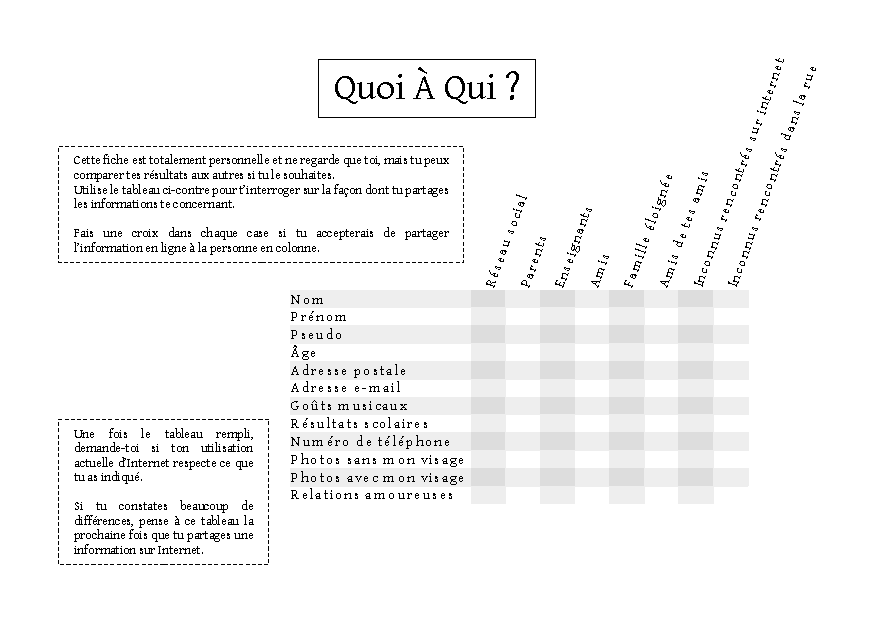
\includepdf[pages={-},fitpaper=false,angle=-90]{activity1.pdf}
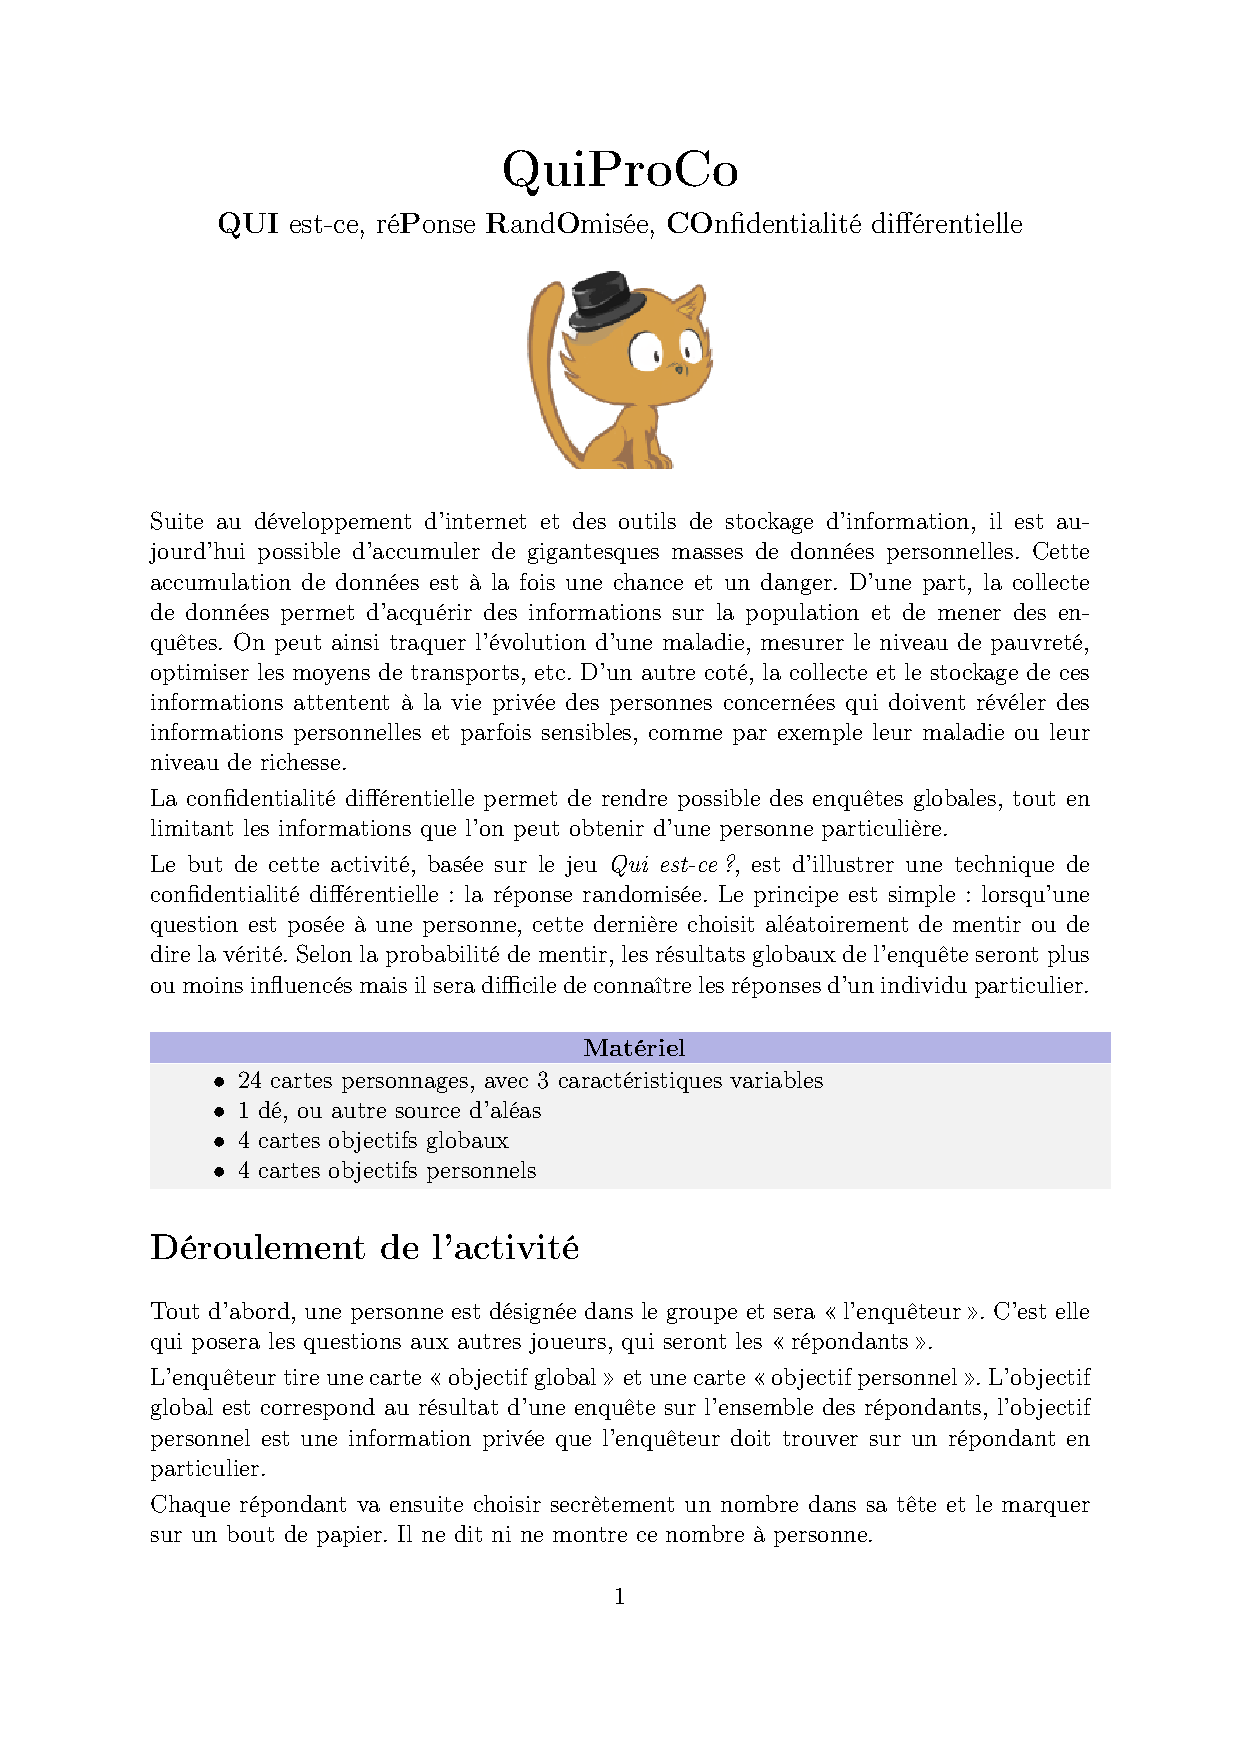
\includepdf[pages={-},fitpaper]{../Qui_est_ce/game.pdf}


\end{document}

